\apendice{Documentación técnica de programación}

\section{Introducción}

\section{Estructura de directorios}

\section{Manual del programador}

\section{Compilación, instalación y ejecución del proyecto}

\section{Pruebas del sistema}

\section{Instalación de herramientas}

\subsection{Virtual Box}
El software de virtualización seleccionado ha sido Oracle VM Virtual Box en su versión 5.1. Este programa ha sido instalado sobre Windows 10, sistema que actúa como anfitrión.

La descarga de este software se puede realizar desde la siguiente dirección web: \url{https://www.virtualbox.org/wiki/Downloads}

\subsection{Ubuntu 16.04}
Como servidor se ha optado por la versión 16.04 de Ubuntu en su versión de escritorio. El sistema ha sido instalado sobre una máquina virtual haciendo uso del software mencionado en la sección anterior.

Para descargar una imagen de este Sistema Operativo se ha de acceder al siguiente enlace: \url{https://www.ubuntu.com/download/desktop}


\subsection{PostgreSQL 9.6 y PgAdmin 3}
PostgreSQL puede ser instalado en Ubuntu desde la consola de comandos. Para ello se han de seguir unos sencillos pasos.
El primer paso es actualizar el repositorio de Ubuntu mediante el siguiente comando sobre la consola:
\begin{lstlisting}
apt-get update
\end{lstlisting}
Ahora se puede comenzar la instalación de Postgres mediante la siguiente línea en la consola de comandos:
\begin{lstlisting}
apt-get install postgresql postgresql-contrib
\end{lstlisting}

Por último, si se desea hacer uso de PgAdmin 3, se podrá instalar mediante el siguiente comando:
\begin{lstlisting}
apt-get install pgadmin3
\end{lstlisting}

Una vez que Postgres ha sido instalado, se ha procedido a la configuración del usuario por defecto (``postgres'') y de la creación de un nuevo usuario ``rs'') para la adición de extensiones y creación de tablas necesarias.

\subsection{PostGIS}
PostGIS es una extensión espacial para las Bases de Datos PostgreSQL. Esta extensión añade soporte para objetos geográficos permitiendo consultas geográficas sobre la Base de Datos.
PostGIS se encuentra distribuido bajo licencia GNU General Public License.

Para instalar PostGIS sobre Ubuntu 16.04 se ha de teclear el siguiente comando:
\begin{lstlisting}
apt-get install postgis
\end{lstlisting}

Se puede obtener más información en la página web oficial de PostGIS: \url{http://www.postgis.net/}.

\subsection{QGIS}
QGIS es una herramienta de información geográfica libre y de código abierto que permite conexiones con PostgreSQL y visualización de los datos obtenidos sobre un mapa físico. También permite la obtención de información geográfica desde Open Street Maps. De esta forma se pueden superponer rutas/trazas obtenidas desde las tablas de la Base de Datos con los mapas de Open Street Maps.

Para instalar QGIS desde ubuntu se han de seguir los pasos mostrados a continuación:

El primer paso es añadir la ruta a los ficheros fuente de QGIS en el fichero ``sources.list'', para ello se puede abrir dicho fichero con el editor nano. Se encuentra en la siguiente ruta: ``etc/apt/''.
Las líneas a añadir son las siguientes y pueden ser incluidas en la parte final del fichero:
\begin{lstlisting}
deb http://qgis.org/debian xenial main
deb-src http://qgis.org/debian xenial main
\end{lstlisting}

Ahora se puede proceder a la instalación de QGIS sobre el Sistema Operativo:

\begin{lstlisting}
apt install qgis python-qgis qgis-plugin-grass
\end{lstlisting}

Una vez instalado, se puede configurar una conexión contra la Base de Datos instalada y configurada anteriormente. Para ello se ha de clicar en el icono de PostgreSQL ubicado en la columna central izquierda. Para ello se han de indicar valores como:

\begin{itemize}
\item \textbf{nombre:} valor que se dará al nombre de la conexión.
\item \textbf{servidor:} servidor contra el que se realizará la conexión. En este caso será el servidor local.
\item \textbf{ de datos:} la Base de Datos de la que serán obtenidos los datos.
\item \textbf{Autenticación:} nombre de usuario y contraseña  del usuario de PostgresQL usado para obtener la información.
\end{itemize}

Para obtener más información sobre QGIS se puede acceder al siguiente enlace: \url{http://www.qgis.org/es/docs/index.html}

\subsection{RouteConverter}
RouteConverter permite visualizar trazas en formato gpx sobre un mapa físico. Es un programa de uso sencillo y rápido.

Para poder usar RouteConverter en la máquina virtual se deberá acceder a la sección de descargas de su plataforma web: \url{http://www.routeconverter.de/downloads/es}. Se puede optar por la versión ''webstart`` o por la versión estable. Para ejecutar ambas se requiere contar con la versión actual de Java.

\section{Manual del usuario}



\subsection{Osmosis}
Osmosis permite extraer una ciudad concreta de un mapa con formato pbf. En el caso de este trabajo, se ha descargado el mapa de España y se ha extraído la ciudad de Burgos. A continuación, se muestran los pasos a dar para obtener un fichero osm.

\subsubsection{Descarga del mapa de España}
Accediendo a la web de descargas de Geofabrik será posible elegir el país cuyo mapa que se desea descargar. Clicando sobre el enlace mostrado en la Figura, se puede descargar el mapa de España en formato pbf.

\subsubsection{Extracción de una ciudad}
Para extraer una ciudad del plano que se acaba de descargar, se ha de abrir la consola del sistema y hacer uso del fichero "getMap.bat". Se necesitarán los siguientes argumentos (entre paréntesis las coordenadas que serán usadas en el caso de Burgos):
\begin{itemize}
	\item Nombre de la ciudad: con esta cadena nombraremos el fichero osm de salida.
	\item Coordenada GPS que indique la parte superior del segmento de mapa que se va a recortar (42.658202).
	\item Coordenada GPS que indique la parte derecha del segmento de mapa que se va a recortar (-3.12561).
	\item Coordenada GPS que indique la parte inferior del segmento de mapa que se va a recortar (41.364442).
	\item Coordenada GPS que indique la parte izquierda del segmento de mapa que se va a recortar (-4.3066641).
\end{itemize}

El comando a teclear constará de lo siguiente:
\begin{itemize}
	\item rb: permite leer el contenido del fichero pbf descargado.
	\item bb: permite extraer los datos indicados en la caja definida por las coordenadas geográficas indicadas a continuación.
	\item top: coordenada geográfica superior.
	\item right: coordenada geográfica derecha.
	\item bottom: coordenada geográfica inferior.
	\item left: coordenada geográfica izquierda.
	\item wx: permite escribir los datos en un fichero osm.
\end{itemize}

Para la ciudad de burgos, el comando será el mostrado en la Figura. Ejecutando el comando se obtendrá el fichero "Burgos.osm".


\subsection{Uso de RouteConverter}

Una vez que se cuenta con este software en el ordenador, se pueden generar rutas o cargar ficheros con rutas ya definidas. En este caso se mostrará cómo cargar los datos de una ruta almacenada en la Base de Datos de Open Street Maps.

El primer paso a dar es la descarga de la traza que se desee visualizar con este programa.

\subsubsection{Descarga de ficheros gpx}
La descarga se realizará desde la página web de Open Street Maps, concretamente en la sección "Trazas". En esta sección se verán las últimas trazas subidas por los usuarios. Eligiendo una traza aleatoria accedemos a la ventana mostrada en la  Figura. Clicando sobre "descargar" se descargará el fichero gpx.

Estos ficheros contendrán una estructura XML con una serie de puntos geográficos que conformarán la ruta seguida por el usuario. La ruta podrá ser identificada con su nombre, el nombre del autor y una breve descripción.

\subsubsection{Carga de ficheros en RouteConverter}

Para cargar la traza en el programa, primero se debe abrir el software y después clicar sobre Archivo, Abrir. En la ventana emergente se ha de seleccionar la traza y clicar sobre Aceptar. En este momento se mostrará la ruta que describe la traza descargada desde Open Street Maps como se aprecia en la Figura \ref{rutaLeonFormigal}.

\begin{figure}[h]
  \centering
    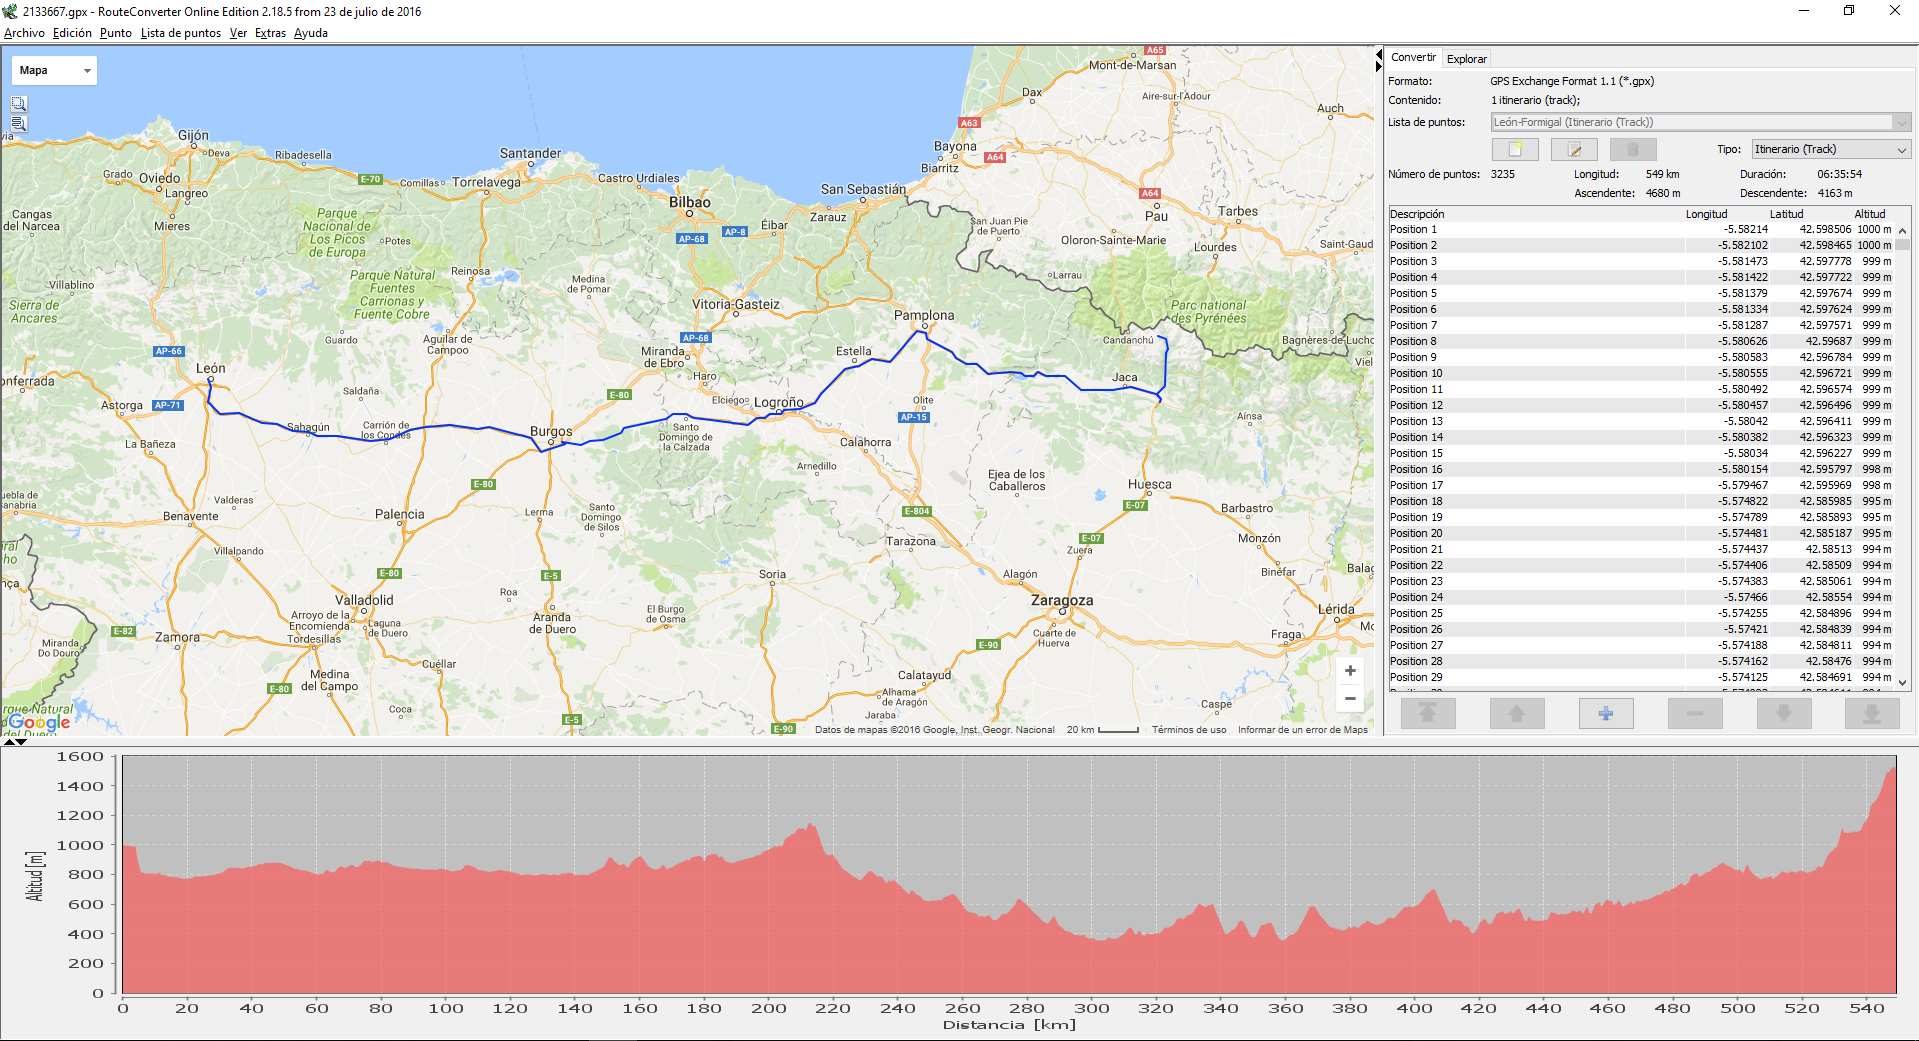
\includegraphics[width=0.8\textwidth]{../img/routeconverter/analisis_traza.png}
  \caption{Ruta desde León a Formigal}
  \label{rutaLeonFormigal}
\end{figure}

En la parte derecha de la ventana se pueden visualizar las rutas detectadas por el programa en el desplegable "Lista de puntos". En la parte inferior se listarán todos los puntos que conforman dicha lista como se ve en la Figura \ref{puntosGeograficos}.

\begin{figure}[h]
  \centering
    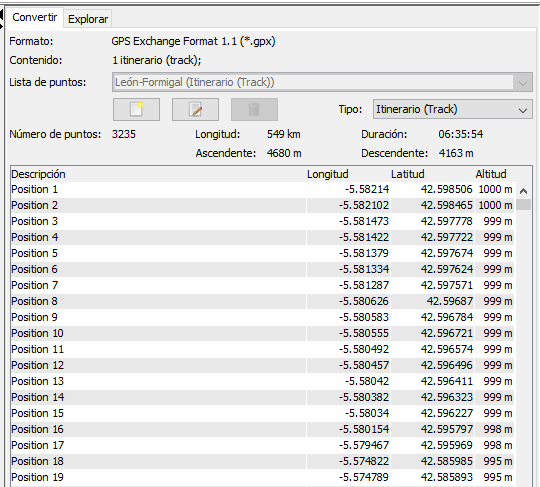
\includegraphics[width=0.6\textwidth]{../img/routeconverter/datos_traza.png}
  \caption{Ruta desde León a Formigal}
  \label{puntosGeograficos}
\end{figure}

Si la traza contiene elevaciones del terreno, se mostrará un perfil en la parte inferior.

